\begin{figure}[t]
    \centering
    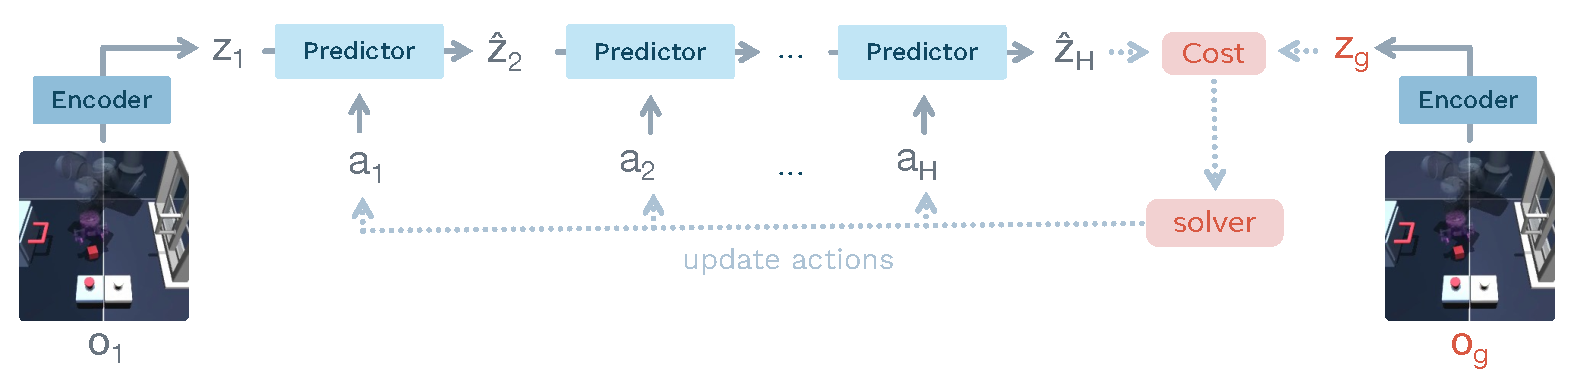
\includegraphics[width=\linewidth]{figs/lewm-plan.pdf}
    \caption{\small \textbf{LeWorldModel Latent Planning.} 
    Given an initial observation $\vo_1$ and a goal $\vo_g$, the world model learned in Fig.~2 performs planning in the LeWM latent space. The initial state embedding $\vz_1$ and the goal embedding $\vz_g$ are obtained from the encoder. The predictor then rolls out future latent states up to a horizon $H$. A latent cost between the final predicted state and the goal embedding guides a solver to optimize the action sequence. This prediction–optimization loop is repeated until convergence to a good plan candidate.}
    \label{fig:lewm}
\end{figure}

\section{Method: LeWorldModel}

In this section, we introduce LeWorldModel (LeWM). We first describe the streamlined training procedure used to learn the latent world model from offline data, including the dataset, model architecture, and training objective. We then explain how the learned model can be leveraged for decision making through latent planning using model predictive control (MPC).


\subsection{Learning the Latent World Model}

\paragraph{Offline Dataset.}
We consider a fully offline and reward-free setting. LeWorldModel is trained solely from unannotated trajectories of observations and actions, without access to reward signals or task specifications. This setup aligns with the JEPA line of work \cite{zhou2025dino-wm,assran2025v}, which aims to learn generic, task-agnostic world models from observational data. Our objective is not to optimize behavior for a specific task, but to learn representations that capture environment dynamics and can later be controlled or adapted to a diverse set of tasks.

The training data consists of trajectories of length $T$ composed of raw pixel observations $\vo_{1:T}$ and associated actions $\va_{1:T}$. Trajectories are collected offline from behavior policies with no optimality requirements; they may be pseudo-expert or exploratory, as long as they sufficiently cover the environment dynamics.
Additional implementation details (batch size, resolution, and sub-trajectory construction) are provided in App.~\ref{appendix:details}.

\paragraph{Model Architecture.} LeWM is built upon two components: an encoder and a predictor. The encoder maps a given frame observation $\vo_t$ into a compact, low-dimensional latent representation $\vz_t$. 
The predictor models the environment dynamics in latent space by predicting the embedding of the next frame observation $\hat{\vz}_{t+1}$ given the latent embedding $\vz_t$ and an action $\va_t$.

\begin{equation}
\begin{aligned}
\text{Encoder:} \quad & \vz_t = \enc(\vo_t) \\
\text{Predictor:} \quad & \hat{\vz}_{t+1} = \pred(\vz_t, \va_t)
\end{aligned}
\tag{LeWM}
\end{equation}

The encoder is implemented as a Vision Transformer (ViT)~\cite{dosovitskiy2020image}. Unless otherwise specified, we use the tiny configuration ($\sim$5M parameters) with a patch size of 14, 12 layers, 3 attention heads, and hidden dimensions of 192. The observation embedding $\vz_t$ is constructed from the \texttt{[CLS]} token embedding of the last layer, followed by a projection step. The projection step maps the \texttt{[CLS]} token embedding into a new representation space using a 1-layer MLP with Batch Normalization~\cite{ioffe2015batchnormalizationacceleratingdeep}. This step is necessary because the final ViT layer applies a Layer Normalization~\cite{ba2016layer}, which prevents our anti-collapse objective from being optimized effectively. 

The predictor is a transformer with 6 layers, 16 attention heads, and 10\% dropout ($\sim$10M parameters). Actions are incorporated into the predictor through Adaptive Layer Normalization (AdaLN)~\cite{peebles2023scalable} applied at each layer. The AdaLN parameters are initialized to zero to stabilize training and ensure that action conditioning impacts the predictor training progressively. The predictor takes as input a history of $N$ frame representations and predicts the next frame representation auto-regressively with temporal causal masking to avoid looking at future embeddings. The predictor is also followed by a projector network with the same implementation as the one used for the encoder.
All components of our world model are learned jointly using the loss described in the following paragraph.

\paragraph{Training Objective.}
Our objective is to learn latent representations useful for predicting the future, i.e., modeling the environment dynamics. {\rm LeWorldModel} training objective is the sum of two terms: a prediction loss and a regularization loss. The prediction loss $\mathcal{L}_{\rm pred}$ (teacher-forcing) computes the error between the predicted embedding of consecutive time-steps:
\begin{equation}
    \mathcal{L}_{\rm pred} \triangleq  \|\hat{\vz}_{t+1} - {\vz}_{t+1}\|^2_2, 
    \quad\quad 
    \hat{\vz}_{t+1} = {\rm pred}_\phi(\vz_t, \va_t).
\end{equation} 
Through the prediction loss, the encoder is incentivized to learn a predictable representation for the predictor.

However, this loss alone leads to representation collapse, yielding a trivial solution in which the encoder maps all inputs to a constant representation. To prevent this behavior, we introduce an anti-collapse regularization term that promotes feature diversity in the embedding space. Specifically, we adopt the Sketched-Isotropic-Gaussian Regularizer (SIGReg)~\cite{balestriero2025lejepa} due to its simplicity, scalability, and stability. SIGReg encourages the latent embeddings to match an isotropic Gaussian target distribution.

Let $\mZ \in \R^{N \times B \times d}$ denote the tensor of latent embeddings collected over the history length $N$, the batch size $B$, and where $d$ demotes the embedding dimension. Assessing normality directly in high-dimensional spaces is challenging, as most classical normality tests are designed for univariate data and do not scale reliably with dimensionality. SIGReg circumvents this limitation by projecting embeddings onto $M$ random unit-norm directions $\vu^{(m)} \in \mathbb{S}^{d-1}$ and optimizing the univariate Epps--Pulley~\cite{epps1983test} test statistic $T(\cdot)$ along the resulting one-dimensional projections $\vh^{(m)} = \mZ \vu^{(m)}$, as illustrated in Fig.\ref{fig:training-framework}. By the Cramér--Wold theorem~\cite{cramer1936some}, matching all one-dimensional marginals is equivalent to matching the full joint distribution.

\begin{equation}
    {\rm SIGReg}(\mZ) \triangleq  \frac{1}{M} \sum_{m=1}^M T(\vh^{(m)}).
\end{equation}

Additional details on SIGReg and the definition of the Epps--Pulley statistical test are provided in appendix \ref{appendix:sigreg}.


The complete LeWM training objective is defined as:
\begin{equation}
\gL_{\rm LeWM} \triangleq \gL_{\rm pred} + \lambda\,{\rm SIGReg}(\mZ).
\end{equation}


The method introduces only two training hyperparameters: the number of random projections $M$ used in SIGReg and the regularization weight $\lambda$. Unless otherwise specified, we use $M = 1024$ projections and $\lambda = 0.1$. In practice, we observe that the number of projections has negligible impact on downstream performance (see Sec.~\ref{sec:exp_control} and App.~\ref{appendix:ablations}), making $\lambda$ the only effective hyperparameter to tune. This greatly simplifies hyperparameter selection, as $\lambda$ can be efficiently optimized using a simple bisection search with logarithmic complexity. We do not employ stop-gradient, exponential moving averages, or additional stabilization heuristics. Gradients are propagated through all components of the loss, and all parameters are optimized jointly in an end-to-end manner, resulting in a streamlined and easy-to-implement training procedure. The training logic is summarized in Alg.~\ref{alg:train-alg}.

\begin{figure}[t]
\centering
\captionsetup{labelformat=empty}
\caption{\textbf{Algorithm \ref*{alg:train-alg}.} Pseudo-code for the training procedure of LeWorldModel. Pixel observations are encoded into latent embeddings, and a predictor estimates the dynamics by predicting the next-step embedding conditioned on actions. The model is optimized end-to-end using a next-embedding prediction loss together with a step-wise SIGReg regularization term to prevent representation collapse.}
\addtocounter{figure}{-1}
\refstepcounter{algorithm}
\label{alg:train-alg}
\begin{tcolorbox}[
  colback=codebg,
  colframe=codebg,
  arc=7pt,
  outer arc=7pt,
  boxrule=0pt,
  left=3pt, right=3pt, top=3pt, bottom=3pt,
  width=0.9\linewidth
]
\begin{lstlisting}[style=pythonstyle]
def LeWorldModel(obs,actions,lambd=0.1):
    """
    obs: (B, T, C, H, W) raw pixels sequence
    actions: (B, T, A) action sequence
    lambd: (float) SIGReg loss weight
    """
    
    emb = encoder(obs) # (B, T, D)
    next_emb = predictor(emb,actions) #(B, T, D)
    
    # -- LeWorldModel training loss
    
    # next-embedding prediction loss
    pred_loss = F.mse_loss(emb[:, 1:] - next_emb[:, :-1])
    
    # step-wise sigreg (anti-collapse)
    sigreg_loss = mean(SIGReg(emb.transpose(0, 1))
    
    return pred_loss + lambd * sigreg_loss
\end{lstlisting}
\end{tcolorbox}
\end{figure}

\subsection{Latent Planning}

At inference time, we perform trajectory optimization in our world model latent space, as illustrated in Fig.\ref{fig:lewm}. Given an initial observation $\vo_1$, we initialize a candidate action sequence randomly and iteratively rollout predicted latent states up to a planning horizon $H$. The model predicts latent transitions according to
\begin{equation*}
\hat{\vz}_{t+1} = \pred(\hat{\vz}_t, \va_t), \quad
\hat{\vz}_1 = \enc(\vo_1),
\end{equation*}
Planning is performed by optimizing the action sequence to minimize a terminal latent goal-matching objective:
\begin{equation}
\gC(\hat{\vz}_H) = \| \hat{\vz}_H - \vz_g \|_2^2, \quad
\vz_g = \enc(\vo_g),
\end{equation}
where $\hat{\vz}_H$ is the predicted latent state at the end of the rollout and $\vz_g$ is the latent embedding of the goal observation $\vo_g$. The world model parameters remain fixed during planning. This procedure corresponds to a finite-horizon optimal control problem:
\begin{equation}
\va^*_{1:H} = \arg\min_{\va_{1:H}} \gC(\hat{\vz}_H),
\label{eq:argmin_plan}
\end{equation}
which we solve using the Cross-Entropy Method (CEM)~\cite{rubinstein2004cross}, a sampling method that iteratively selects the best plan and updates the parameters of the sampling distribution with the statistics of the best plans. The planning horizon $H$ trades off long-term lookahead against increased computational cost and model bias. In particular, auto-regressive rollouts accumulate prediction errors as the horizon grows, which can deteriorate the quality of the optimized action sequence. To mitigate this effect, we adopt a Model Predictive Control (MPC) strategy: only the first $K$ planned actions are executed before replanning from the updated observation.
We provide more details on the planning strategy in appendix~\ref{appendix:details}.
